

\section{Диаграммы цвет-интенсивность}

Если построить диаграмму цвет-интенсивность \ref{fig:color-magnitude}, то можно увидеть, насколько отличается блеск кандидатов от блеска остальных источников в области и от эталонной выборки. Видно, что звёзды выборки гораздо ярче как кандидатов, так и всех звёзд области. 

Большинство кандидатов очень слабые, их звёздные величины находятся на грани чувствительности GALEX. Также видно, что цвет FUV-NUV у кандидатов может быть отрицательным, и также просто отличаться от эталонных. Это даёт представление о количестве кандидатов, пришедших в выборку с третьим, неультрафиолетовым критерием.

Источников на рисунке \ref{fig:color-magnitude} меньше, чем в итоговом списке, так как многие как кандидаты, так и остальные звёзды не имеют FUV измерений.

\begin{figure}[ht]
\center{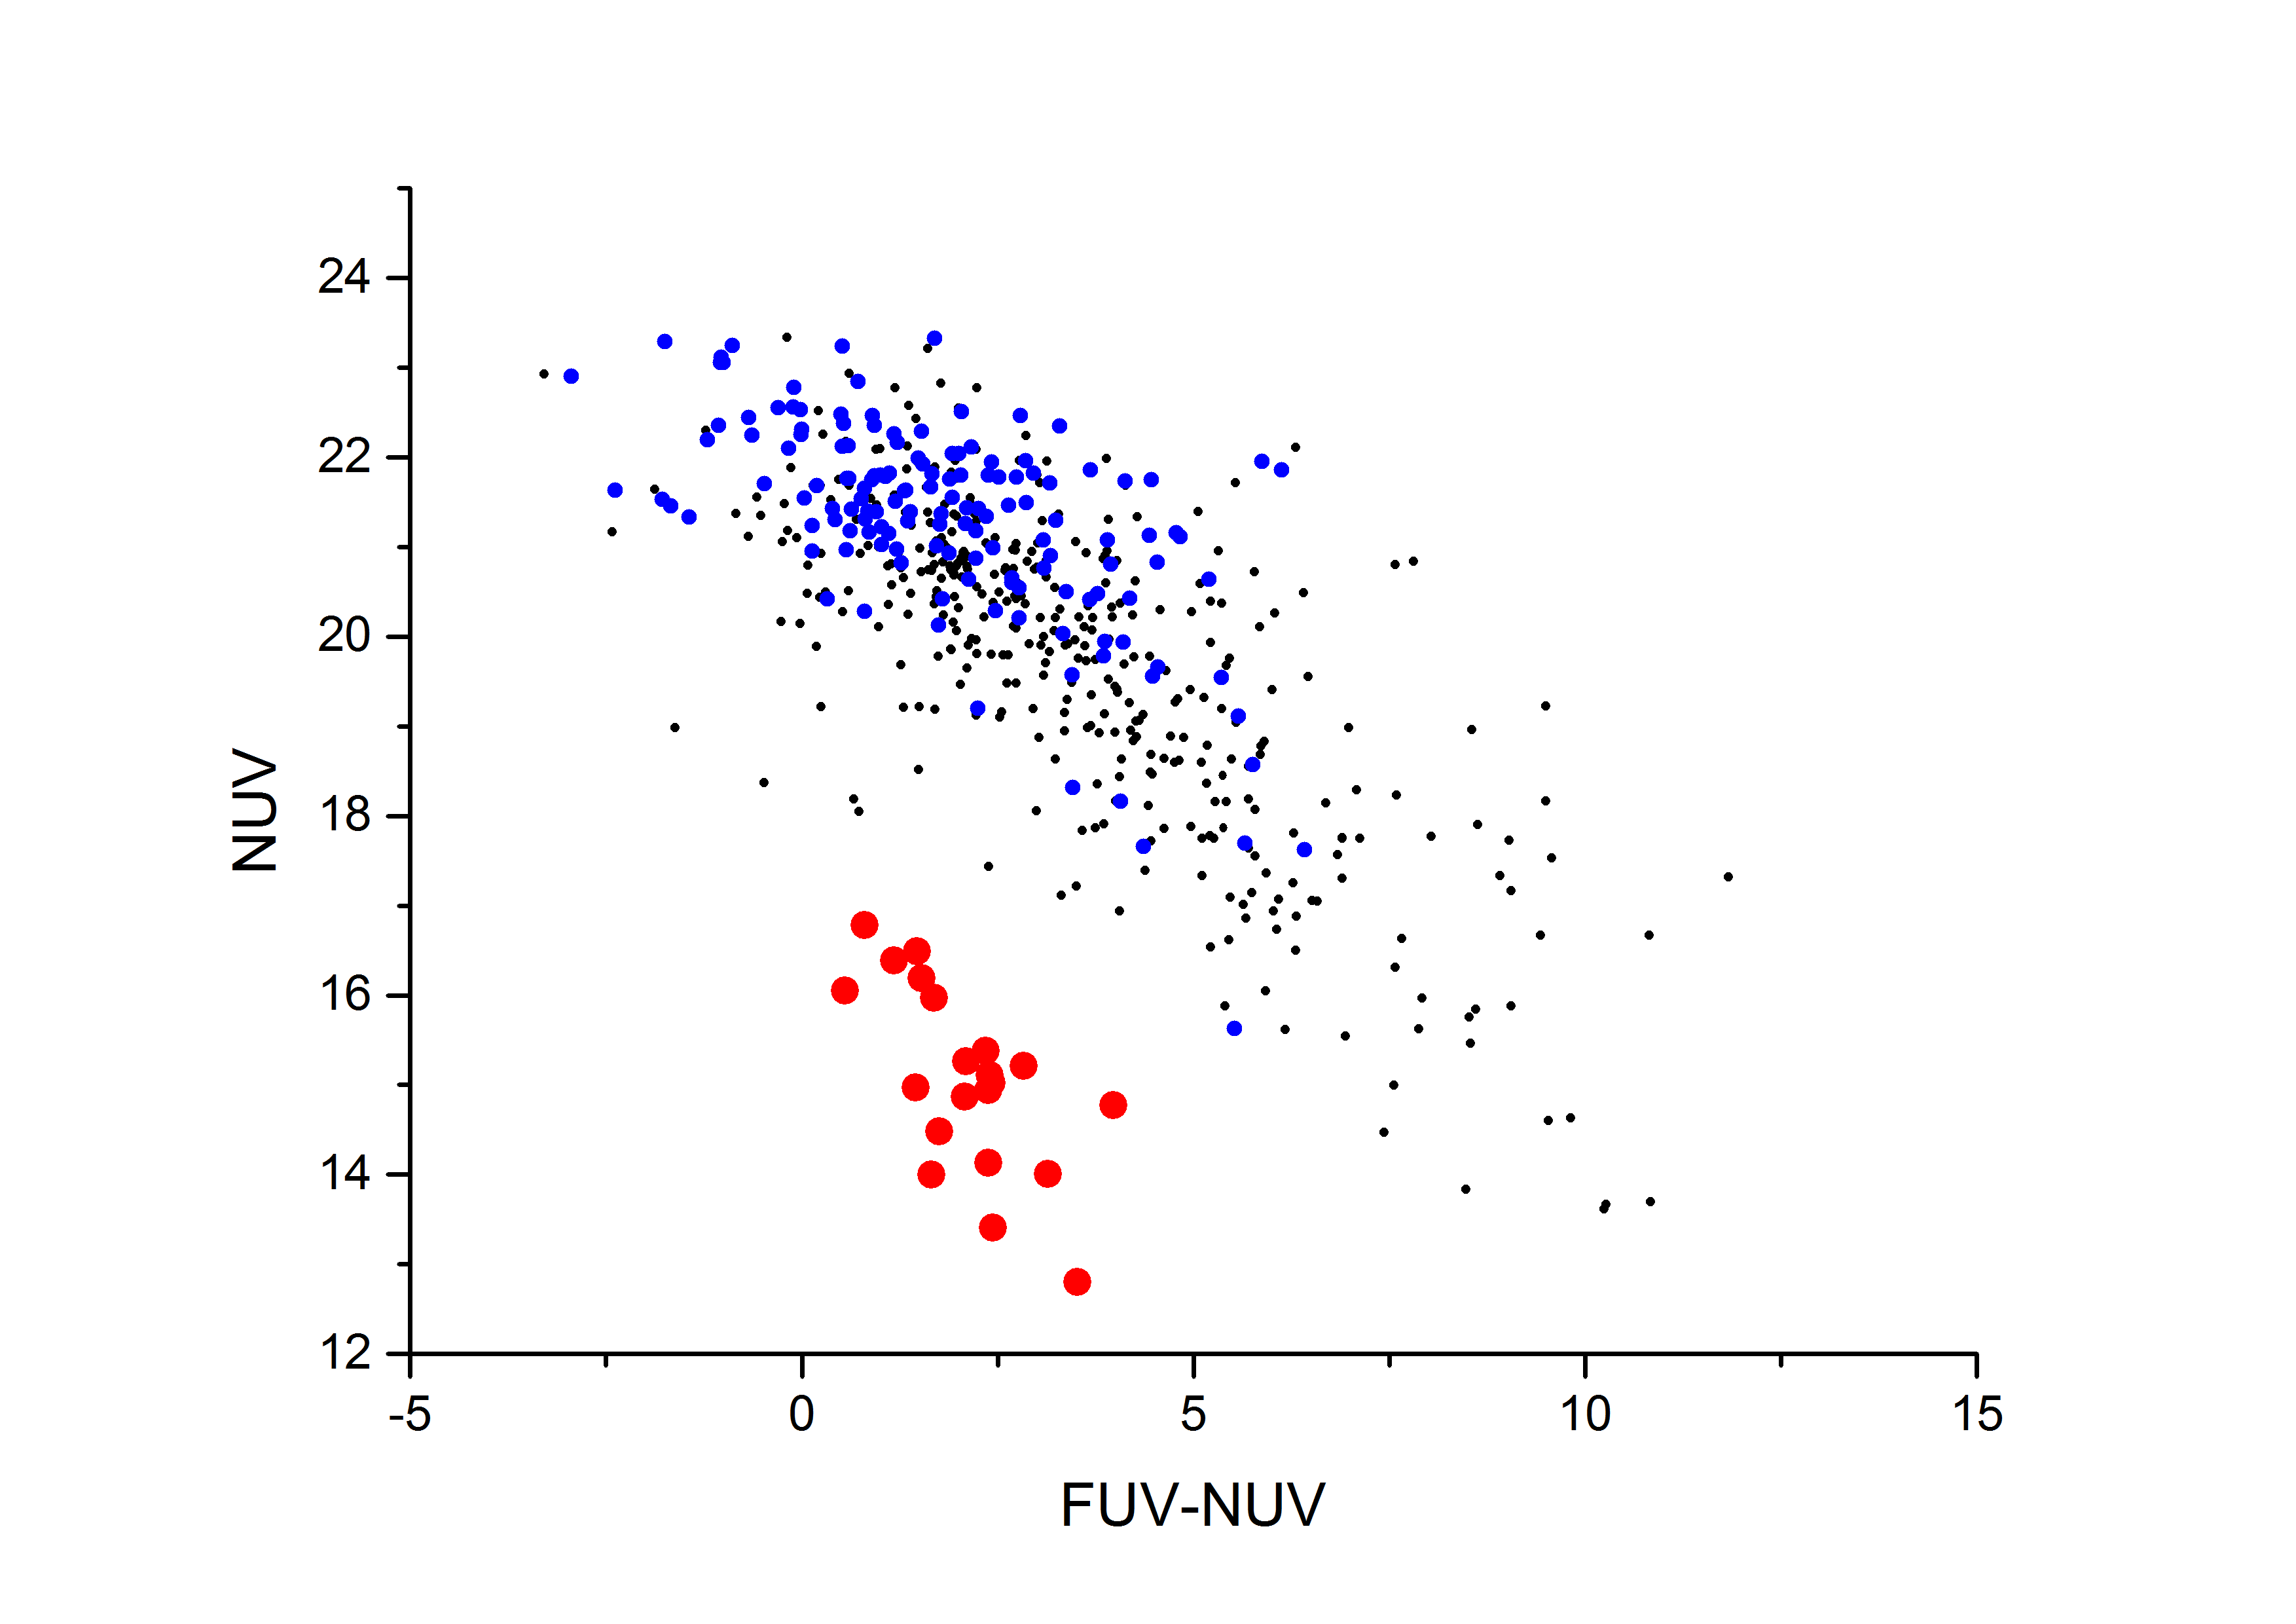
\includegraphics[width=0.6\linewidth]{colormagnitude.png}}
\hfill
\caption{Диаграмма цвет-интенсивность. Красным отмечены звёзды эталонной выборки, синим -- отобранные кандидаты}
\label{fig:color-magnitude}
\end{figure}

\section{Распределение спектральной энергии}

Сервис VOSA, использовавшийся для оценки эффективных температур, может строить распределение спектральной энергии, SED. Мы можем построить такую характеристику для эталонных звёзд, например, для T Tau, которая также входит в этот список, и сравнить с ней SED кандидатов. 

Как видно из рисунка, распределения не всегда похожи. Однако у большинства кандидатов в ультрафиолетовом диапазоне присутствует пик, подобный пику у T Tau.

\begin{figure}[ht]
\begin{minipage}[ht]{0.49\linewidth}
\center{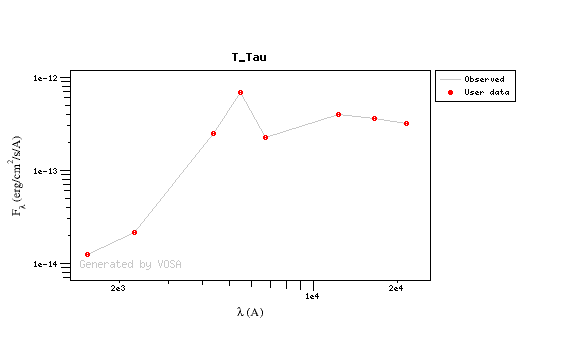
\includegraphics[width=1\linewidth]{T_Tau.png} \\ }
\end{minipage}
\hfill
\begin{minipage}[ht]{0.49\linewidth}
\center{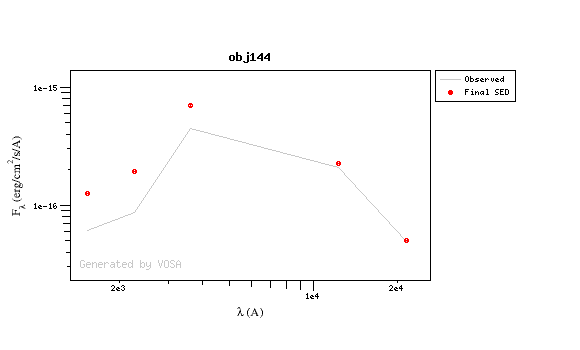
\includegraphics[width=1\linewidth]{obj144.png} \\ }
\end{minipage}
\begin{minipage}[ht]{0.49\linewidth}
\center{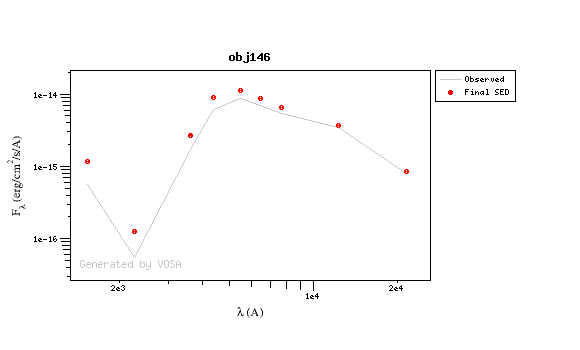
\includegraphics[width=1\linewidth]{obj146.png} \\ }
\end{minipage}
\hfill
\begin{minipage}[ht]{0.49\linewidth}
\center{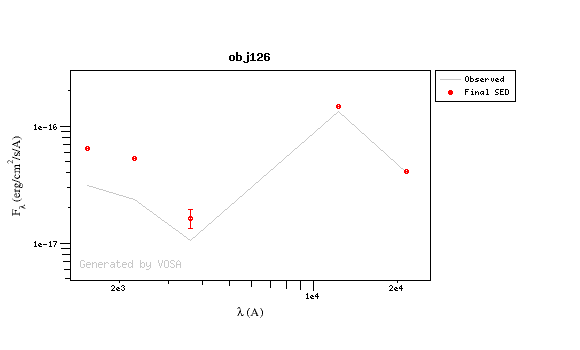
\includegraphics[width=1\linewidth]{obj126.png} \\ }
\end{minipage}
\caption{Распределение спектральной энергии (SED) для T Tau и некоторых из кандидатов}
\label{fig:sed}
\end{figure}

\section{Оценка поглощения}
Надо доделать.
в (Far-ultraviolet Observation of the Aquila Rift with FIMS SPEAR) упоминается, что E(B-V) < 0.3.

Межзвёздное поглощение в исследуемой области определяется в основном наличием молекулярных облаков. Однако, наблюдения миссии GALEX относятся только к периферии этих облаков, где поглощение значительно ниже. По некоторым оценкам, его величина $A_v < 0.5$ [Ana Ines], и таким поглощением можно пренебречь.

\section{Расположение}
Картинки с координатами и собственными движениями.

\section{Классические и со слабыми линиями}
Что они распределены по гауссу и вдоль прямой соответственно, если смотреть на диаграмму FUV-NUV vs J-K. Вообще распредедить кандидаты в группы по WTTS, CTTS и просто TTS.
